\documentclass[12pt]{article}

% ----------------------------------------------------------------------
% Definir packages externos, língua, margens, tipos de letra, novos 
% comandos e cores
% ----------------------------------------------------------------------
\usepackage[utf8]{inputenc} % Codificação utilizada
\usepackage[english]{babel} % Idioma de escrita

\usepackage[export]{adjustbox} % Alinhar imagens
\usepackage{amsmath} % Comandos extra para escrita matemática
\usepackage{amssymb} % Símbolos matemáticos
\usepackage{anysize} % Personalizar as margens
    \marginsize{2cm}{2cm}{2cm}{2cm} % {esquerda}{direita}{cima}{baixo}
\usepackage{appendix} % Apêndices
\usepackage{cancel} % Cancelar expressões
\usepackage{caption} % Legendas
    \DeclareCaptionFont{newfont}{\fontfamily{cmss}\selectfont}
    \captionsetup{labelfont={bf, newfont}}
\usepackage{cite} % Citações, tipo [1 - 3]
\usepackage{color} % Colorir texto
\usepackage{fancyhdr} % Cabeçalho e rodapé
    \pagestyle{fancy}
    \fancyhf{}
    \fancyhead[L]{\footnotesize\fontfamily{cmss}\selectfont IST} % Esquerda do cabeçalho
    \fancyhead[R]{\footnotesize\fontfamily{cmss}\selectfont ULisboa} % Direita do cabeçalho
    \fancyfoot[L]{\footnotesize\fontfamily{cmss}\selectfont Projeto de Sistemas Digitais} % Esquerda do rodapé
    \fancyfoot[C]{\thepage} % Centro do rodapé
    \fancyfoot[R]{\footnotesize\fontfamily{cmss}\selectfont LEEC} % Direita do rodapé
    \renewcommand{\footrulewidth}{0.4pt} % Régua do rodapé
\usepackage{float} % Utilizar o especificador [H] nas figuras
\usepackage{graphicx} % Imagens em LaTeX
\usepackage[colorlinks = true, plainpages = true, linkcolor = istblue, urlcolor = istblue, citecolor = istblue, anchorcolor = istblue]{hyperref}
\usepackage{indentfirst} % Primeiro parágrafo
\usepackage{siunitx} % Unidades SI
\usepackage{subcaption} % Subfiguras
\usepackage{titlesec} % Tipo de letra
    \titleformat{\section}{\fontfamily{cmss}\selectfont\Large\bfseries}{\thesection}{1em}{}
    \titleformat{\subsection}{\fontfamily{cmss}\selectfont\large\bfseries}{\thesubsection}{1em}{}
    \titleformat{\subsubsection}{\fontfamily{cmss}\selectfont\normalsize\bfseries}{\thesubsubsection}{1em}{}
    \fancyfoot[C]{\fontfamily{cmss}\selectfont\thepage}

% Encher de texto aleatório (apagar)
\usepackage{lipsum}
\usepackage{duckuments}
\usepackage[table]{xcolor}

% Novos e renovar comandos
\newcommand{\sen}{\operatorname{\sen}} % Definição da função seno
\newcommand{\HRule}{\rule{\linewidth}{0.5mm}} % Definição de uma régua
\renewcommand{\appendixpagename}{\LARGE \fontfamily{cmss}\selectfont Apêndices}
\renewcommand{\appendixtocname}{Apêndices}

% Cores
\definecolor{istblue}{RGB}{3, 171, 230}
\definecolor{dkgreen}{rgb}{0,0.6,0}
\definecolor{gray}{rgb}{0.5,0.5,0.5}

%%%%%%%%%%%%%%%%%%%%%%%%%%%%%%%%%%%%%%%%%%%%%%%%%%%%%%%%%%%%%%%%%%%%%%%%
%                               Documento                              %
%%%%%%%%%%%%%%%%%%%%%%%%%%%%%%%%%%%%%%%%%%%%%%%%%%%%%%%%%%%%%%%%%%%%%%%%
\begin{document}

% ----------------------------------------------------------------------
% Capa
% ----------------------------------------------------------------------
\begin{center}
    \begin{figure}
        \vspace{-1.0cm}
        
\includegraphics[scale = 0.3, left]{Imagens/IST_A.eps} % Tipo de assinatura do IST
    \end{figure}
    \mbox{}\\[2.0cm]
    \textsc{\Huge Projeto de Sistemas Digitais}\\[2.5cm]
    \textsc{\LARGE MEEC}\\[2.0cm]
    \HRule\\[0.4cm]
    {\large \bf {\fontfamily{cmss}\selectfont Computing Determinants : Scheduling and Resource Sharing} [\texttt{EN}]}\\[0.2cm]
    \HRule\\[1.5cm]
\end{center}

\begin{flushleft}
    \textbf{\fontfamily{cmss}\selectfont Authors:}
\end{flushleft}

\begin{center}
    \begin{minipage}{0.4\textwidth}
        \begin{flushleft}
            Alexandre Santos (99884)\\
            Nuno Abreu (103416)\\
            Carlos Reis nº103166 \\
        \end{flushleft}
    \end{minipage}%
    \begin{minipage}{0.6\textwidth}
        \begin{flushright}
            \href{mailto:ares.santos@tecnico.ulisboa.pt}{\texttt{ares.santos@tecnico.ulisboa.pt}}\\
            \href{mailto:nuno.g.tribolet.de.abreu@tecnico.ulisboa.pt}{\texttt{nuno.g.tribolet.de.abreu@tecnico.ulisboa.pt}}\\
            \href{mailto:guilherme.garcia@tecnico.ulisboa.pt}{\texttt{guilherme.garcia@tecnico.ulisboa.pt}}\\
            
        \end{flushright}
    \end{minipage}


\end{center}
    
\begin{flushleft}
    \large $\boxed{\text{\bf \fontfamily{cmss}\selectfont Group 10}}$\\[4.0cm]
\end{flushleft}
    
\begin{center}
    \large \bf \fontfamily{cmss}\selectfont 2024/2025 -- 1st Semester, P1
\end{center}

\thispagestyle{empty}

\setcounter{page}{0}

\newpage

% ----------------------------------------------------------------------
% Conteúdo
% ----------------------------------------------------------------------


\section{Introduction}
The following report pertains to the second laboratory task of Project of Digital Systems.

The objective is to design a program that computes determinants utilizing
scheduling and resource Sharing, with VHDL hardware description language and making use of simulation and logic synthesis. 

\section{Data-flow Graph}
To start the work a data-flow graph was made accordingly with the operations needed to compute the determinant's. The result is presented in image \ref{fig:data} corresponds to one loop iteration of the algorithm. This graph shows the serialization limitation of the sequence of operations needed and allows us to make a priority list based on the critical path.

\begin{figure}[H]
	\centering
	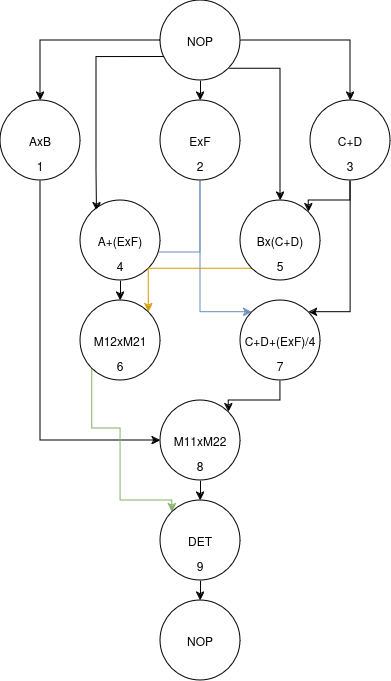
\includegraphics[width=0.35\linewidth]{Imagens/flowdat.drawio.png}
	\caption{Data-Flow Graph}
	\label{fig:data}
\end{figure}

\section{Priority List}
Using the critical path as metric the priority list was made and is represented in \ref{tab:list}. Utilizing this resource we can a choose of scheduling process that depends on the importance of each process and the resources available.

\begin{table}[H]
	\center
	\begin{tabular}{|c|c|c|}
		\hline
		  Nº & Operation & Priority \\
		\hline
		1 & mul & 3 \\
		\hline
        2 & mul & 4 \\
		\hline
        3 & add & 4 \\
		\hline
        4 & add & 3 \\
		\hline
        5 & mul & 3 \\
		\hline
        6 & mul & 2 \\
		\hline
        7 & add & 3 \\
		\hline
        8 & mul & 2 \\
		\hline
        9 & sub & 1 \\
		\hline
	\end{tabular}
    \begin{tabular}{|c|c|c|}
		\hline
		  Nº & Operation & Priority \\
		\hline
        2 & mul & 4 \\
        \hline
        3 & add & 4 \\
		\hline
        1 & mul & 3 \\
		\hline
        4 & add & 3 \\
		\hline
        5 & mul & 3 \\
		\hline
        7 & add & 3 \\
        \hline
        6 & mul & 2 \\
		\hline
        8 & mul & 2 \\
		\hline
        9 & sub & 1 \\
		\hline
	\end{tabular}
	\caption{Priority List}
	\label{tab:list}
\end{table}
\section{List Scheduling}
With the information obtained from the Priority List \ref{tab:list}. Considering that each operation requires a clock cycle and the only resources available (for arithmetic operations) are: 2 multipliers and 1 ALU (addition and subtraction). The list scheduling was done as can be seen in image \ref{fig:sch}, having all the constraints in mind and applying ASAP.

\begin{figure}[H]
	\centering
	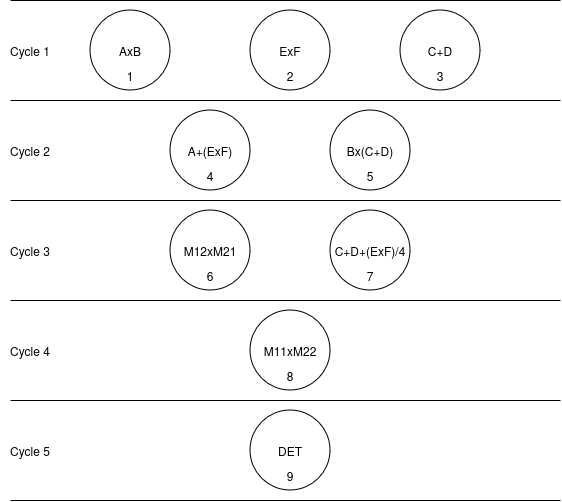
\includegraphics[width=0.55\linewidth]{Imagens/stop.drawio.png}
	\caption{Data-Flow Graph}
	\label{fig:sch}
\end{figure}


<<<<<<< HEAD
Each state takes up one clock cycle, except for the done state which extends indefinitely. A reset signal returns the control to the first state, the counter to 0 and all registers to 0.

\begin{figure}[H]
	\centering
	\includegraphics[width=0.55\linewidth]{images/FSM_lab2.drawio.png}
	\caption{Finite State Machine}
	\label{fig:fsm}
\end{figure}
=======
>>>>>>> 0e5e12d8d255503de26a2fa39376da1a2be4ba90

\section{Circuit Design}
\subsection{Data-Path}
To perform all the operation we designed the data-path for the circuit. In order to be efficient and use the least amount of different components we organized the data-path as can be seen in image \ref{fig:path}. 

All register's , excluding register6, have multiplexers in their entry's to choose between memory and the operations components outputs. Register6 doesn't have a multiplexer because no value will be saved other then the letter F from memory. To better understand our implementation the table \ref{tab:reg} was made, where the register values saved in the registers are explicit.

The operation components also have some multiplexers in their entrances. Mul1 only as one multiplexers in one of the entrances because the operation were organized in other that all multiplications are made with at least the value saved in register2. 

Mul2 doesn't have any multiplexers because as can be seen in our data-flow graph there is only one time where there is two multiplications at the same time.

The ALU is the component that performs more operations with different registers so two multiplexers are needed to perform all operations.

\begin{figure}[H]
	\centering
	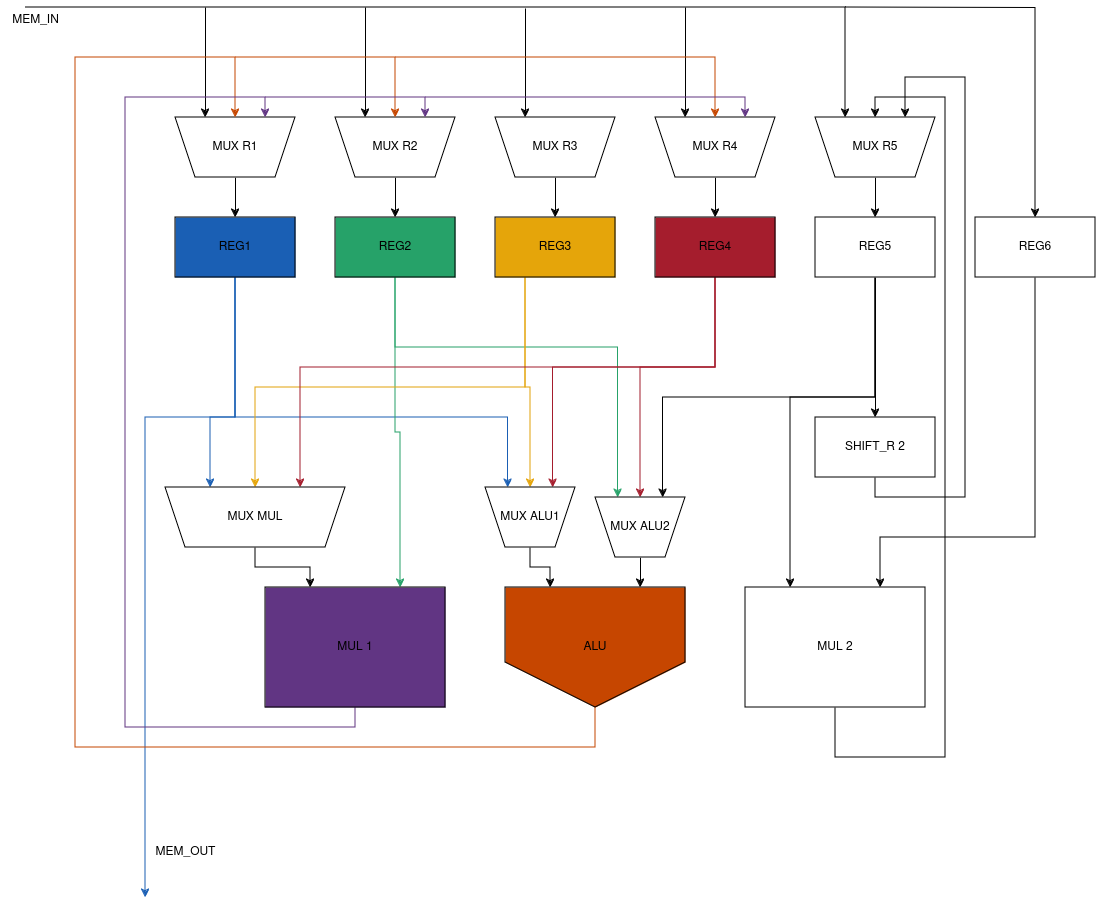
\includegraphics[width=0.7\linewidth]{Imagens/Datapath.png}
	\caption{Data-Path Graph}
	\label{fig:path}
\end{figure}

\begin{table}[H]
	\center
	\begin{tabular}{|c|c|c|c|c|c|c|}
		\hline
		Cycle & 0 & 1& 2&3&4&5\\
        \hline
        R1 &A&A&M12&M12xM21&M12xM21&Det\\
        \hline
        R2 &B&B&M21&M22&M22xM11&M22xM11\\
        \hline
        R3&C&M11&M11&M11&M11&M11\\
        \hline
        R4&D&C+D&C+D&C+D&C+D&C+D\\
        \hline
        R5&E&ExF&(ExF)/4&(ExF)/4&(ExF)/4&(ExF)/4\\
        \hline
        R6&F&F&F&F&F&F\\
        \hline
	\end{tabular}
	\caption{Register values}
	\label{tab:reg}
\end{table}

\subsection{Control Unit}
The control unit implements a finite state machine with 5 states for each of the cycles in the list scheduling plus two states for loading data from memory($st0$ and $st0\_1$) and one for after all computations are complete where a "done" signal is produced. A single counter is incremented to iterate over the full memory.

Each state takes up one clock cycle, except for the done state which extends indefinitely. A reset signal returns the control to the first state, the counter to 0 and all registers to 0.

\begin{figure}[H]
	\centering
	\includegraphics[width=0.55\linewidth]{Imagens/FSM_lab2.drawio.png}
	\caption{Finite State Machine}
	\label{fig:fsm}
\end{figure}
\section{Simulation and verification}

For simplicity, we will only show the simulations done for MemIn1.

The test-bench used is very simple. All it does is reset the circuit followed by handling the clock.

The clock cycle of the circuit was set to 18ns in the constraints and the same value was used for the test-bench. This left us with a WNS of 3.697ns.

\begin{figure}[H]
	\centering
	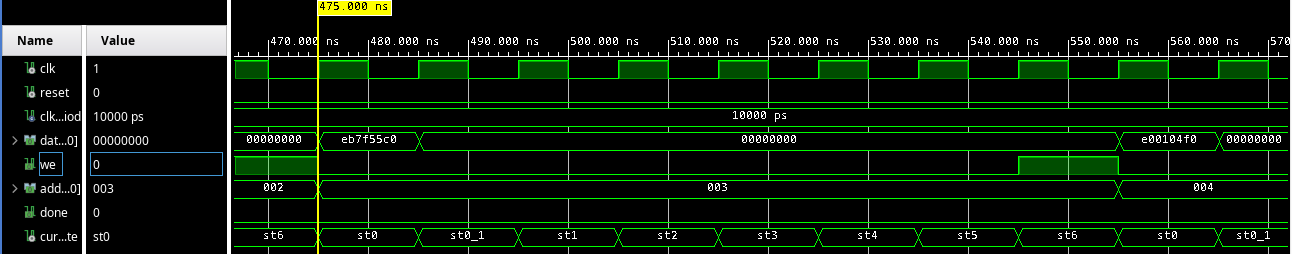
\includegraphics[width=0.7\linewidth]{Imagens/Behavioral.png}
	\caption{Behavioral simulation}
	\label{fig:behav}
\end{figure}

Figure \ref{fig:behav} is a portion of the behavioral simulation of the circuit. We can observe the different states and the data out change as the calculations finish and write enable toggles. Notice also how this is address 3 of the memory, the final value of -536804112 is correct.


\begin{figure}[H]
	\centering
	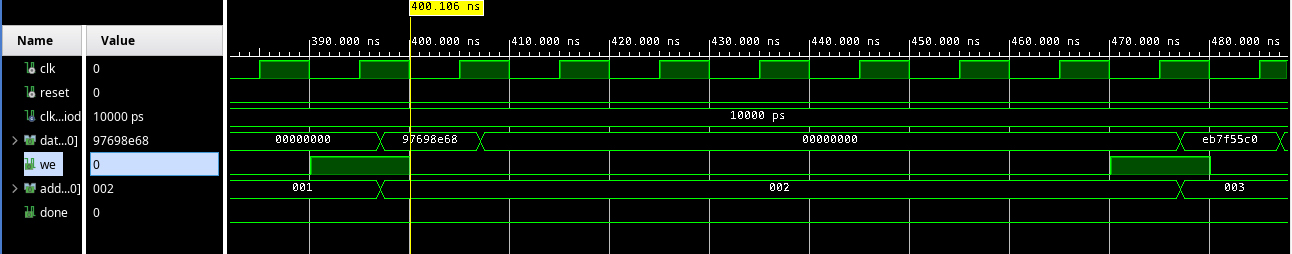
\includegraphics[width=0.7\linewidth]{Imagens/PostImplementation.png}
	\caption{Post Implementation Timing Simulation}
	\label{fig:PImple}
\end{figure}

Figure \ref{fig:PImple} is a similar cutout, but now from the Post-Implementation Timing Simulation. We now can't see the states, however we can see that the write enable and data out behaviour is the same. Notice how the result of -343976512 is correct for address 2.

\section{Pipeline}

We can in fact improve the circuit by employing pipeline. Using at least 5 MULs and 4 ALUs. We also need an extra 11 registers, but we no longer employ multiplexers.
We can expect to go from a result every 7 clock cycles to a result every clock cycle. Over the given data set that would result in the 16 determinants being available after 25 clock cycles, that is 450. Without pipelining it would be 2016ns.

\begin{figure}[H]
	\centering
	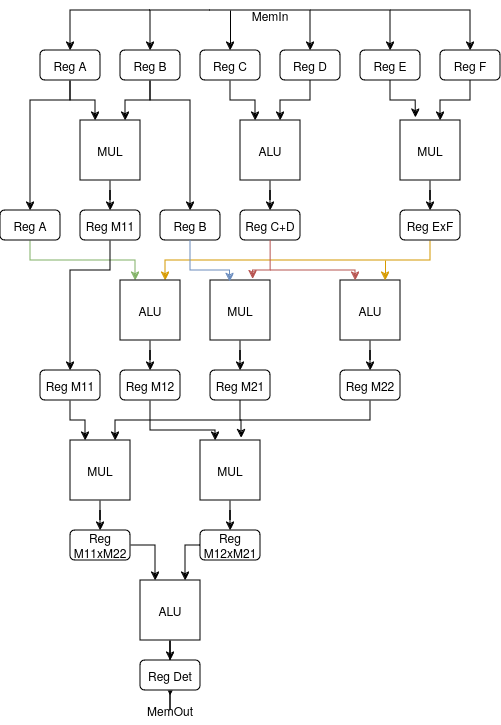
\includegraphics[width=0.7\linewidth]{images/pipe.png}
	\caption{Draft block diagram of the pipeline datapath}
	\label{fig:pipe}
\end{figure}

\section{Conclusion}
Through this laboratory we successfully simulated a datapath, control unit(with one counter for address tracking) components and memory access.

The focus of this project was to design a datapath in an efficient way, sharing physical resources(components) between various operations and reusing registers for holding different signals. This was achieved through priority listing and list scheduling.
  
We simulated the final circuit to test if its behaviour was as designed. This allowed us to
find errors in our design, correct them in timely manner and fine tune the clock period to a reasonable value maintaining a positive Worst Negative Slack.

Further optimizations were discussed such as pipelining and reducing the number of registers. Both solutions implied a trade-off, the former requiring more components and the latter increasing the clock period thus decreasing throughput.


\end{document}
